\documentclass[conference]{IEEEtran}

\usepackage[utf8]{inputenc}
\usepackage[T1]{fontenc}
\usepackage{silence}\WarningsOff[latexfont]

\usepackage{amsmath}

\RequirePackage{tikz}[2010/10/13]
\usetikzlibrary{arrows,automata,calc,intersections,patterns,decorations.pathmorphing,decorations.pathreplacing}

\usepackage{graphicx}
\usepackage{cite}
\usepackage{url}
\usepackage[caption=false,font=footnotesize]{subfig}
\usepackage[binary-units,per-mode=symbol]{siunitx}
\sisetup{list-final-separator = {, and }}
\usepackage{booktabs}
\usepackage{pifont}
\usepackage{microtype}
\usepackage{textcomp}
\usepackage[american]{babel}
\usepackage[noabbrev,capitalise]{cleveref}
\usepackage{xspace}
\usepackage{hyphenat}
\usepackage[draft,inline,nomargin,index]{fixme}
\fxsetup{theme=color}
\usepackage{grffile}
\usepackage{xfrac}
\usepackage{multirow}
\RequirePackage{xstring}
\RequirePackage{xparse}
\RequirePackage[index=true]{acro}
\usepackage{float}
\NewDocumentCommand\acrodef{mO{#1}mG{}}{\DeclareAcronym{#1}{short={#2}, long={#3}, #4}}
\NewDocumentCommand\acused{m}{\acuse{#1}}
\usepackage{upquote}

\acrodef{WSN}{Wireless Sensor Network}
\acrodef{MANET}{Mobile Ad Hoc Network}
\acrodef{ROI}{Region of Interest}{short-indefinite={an}, long-plural-form={Regions of Interest}}

\begin{document}

\title{Python Simulator Extension}

\author{
	\IEEEauthorblockN{Rodrigo Joni Sestari, Mat. number 179020}
	\texttt{rodrigo.sestari@unitn.it}
}

\maketitle

\begin{abstract}
This document describes the modifications made to the implementation of Trivial Carrier Sensing and analyses the results.

\end{abstract}

\acresetall

\section{Introduction}
\label{sec:introduction}

\begin{itemize}
\item general objective this document explain the  extending of  simulator framework using the concepts of DES.
\item problem: extend the protocol including a simple carrier sensing function that prevents transmission if there are packets being transmitted within the communication range of the node. The packet is transmitted when the channel becomes free.
\item strategy: create a new state on protocol that represents the trivial Carrier Sensing.
\end{itemize}

\section{Base information}

The protocol is composed by 4 states;\textit{ IDLE, TX, RX, and PROC} where: 
\begin{itemize}
\item IDLE: the node \textit{Thinks} the channel is free	.
\item TX: the node is currently transmitting a packet.
\item RX: the node is currently receiving one or more packets. 
\item PROC: the node is performing a little processing after a TX or an RX.
\end{itemize}

 

The network used to evaluate the extension simulator is composed by 10 nodes, in the Figure 1 show how the network is distributed.
\begin{figure}[H]
	\centering
	\subfloat{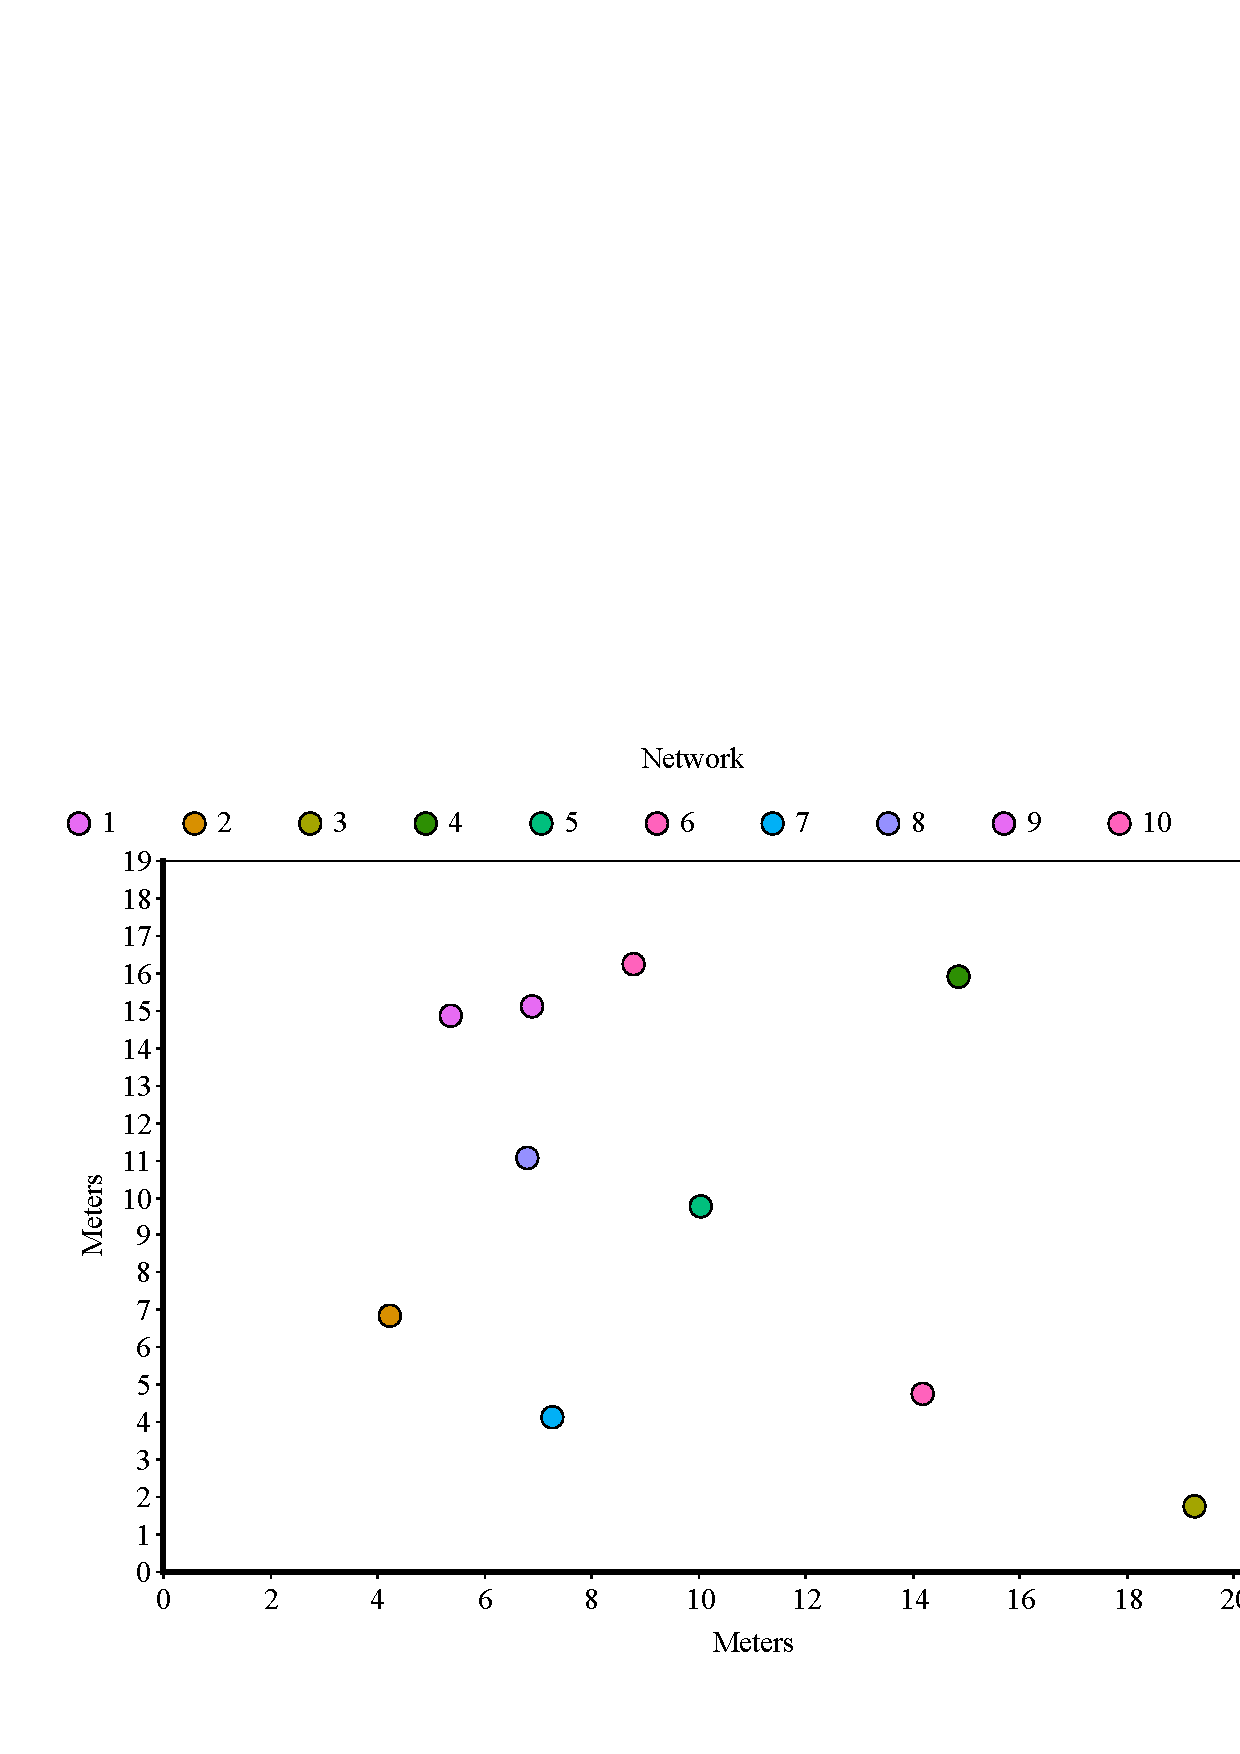
\includegraphics[width=\columnwidth]{figures/net.pdf}}
	\caption{Network}
\end{figure}


\section{Implementation}
 
The implantation consists in create a new state on protocol to simulate the Carrier Sense, This new state is called \textit{CS}, the main idea is that at moment that arrives some packet to transmit, the protocol verify if there any signal in the air, if positive, then the protocol state becomes \textit{CS}, once in the state of \textit{CS}, the protocol change the state when there is not signal the in air.
Is possible see a sample of state machine of protocol in the Figure 2, the red color represent the extension protocol released by this project.


\begin{figure}[ht]
		\centering	
		\subfloat{\label{fig:sm}\includegraphics[width=\columnwidth]{figures/stateMachine.pdf}}
		\caption{State Machine protocol}
\end{figure}

To extent the protocol was necessary modificate three events, bellow will be describe the single modification for each events. The first event that will be described is \textit{end-Proc}, visible on Figure 3, this state is used by a node to know when processing is over, the modification was realised at moment that the queue is not empty, is controlled if there is any signal in the air, in positive case, then the state is changed to \textit{CS}, in negative case the protocol put the packet on the queue. 

\begin{figure}[H]
	\centering
	\subfloat{\label{fig:ep}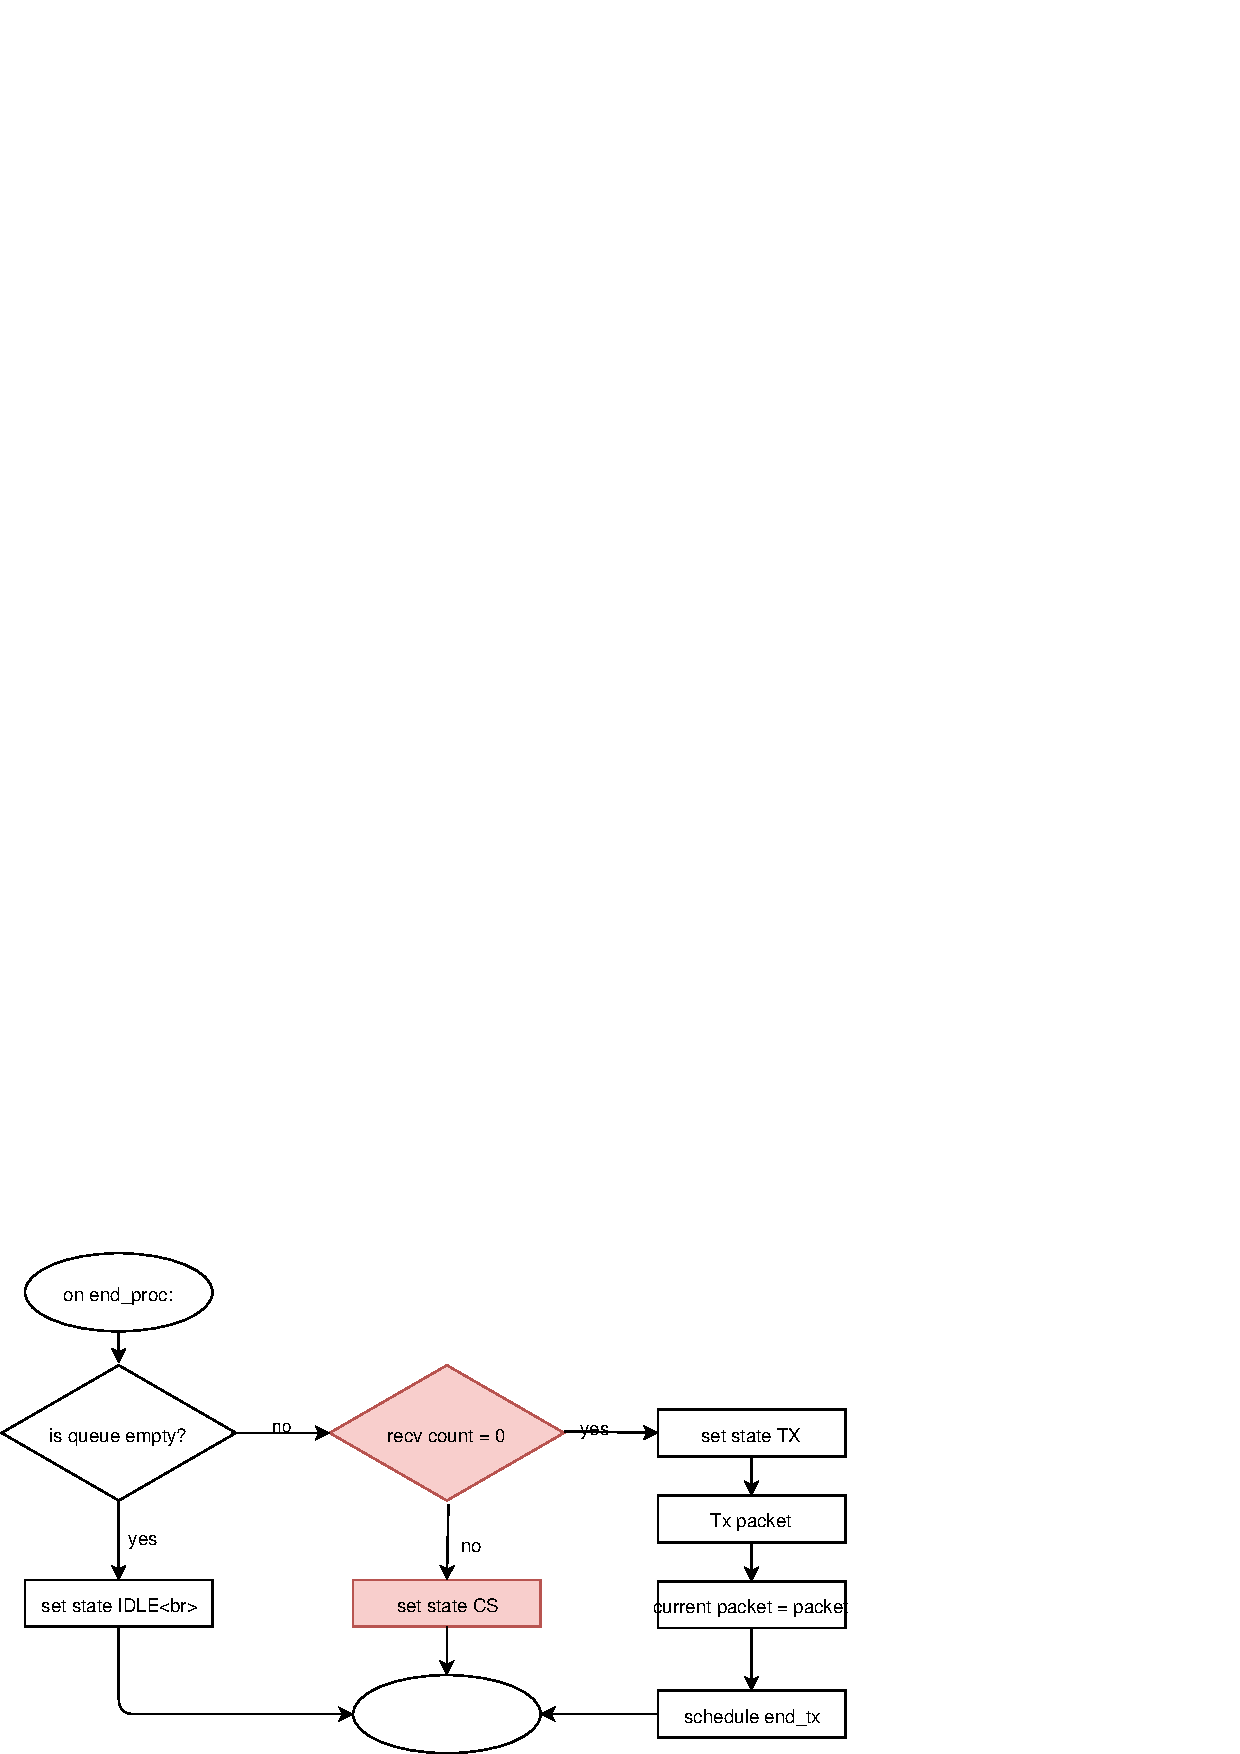
\includegraphics[width=\columnwidth]{figures/end_proc.pdf}}
	\caption{end-Proc event}
\end{figure}

 The next event is \textit{end-Rx}, visible in the Figure 4, this event notifies the node the end of an incoming packet. The modification created in the extension protocol is concentrated on \textit{CS} state when there is no signal in the air, in this case, the state is changed to \textit{TX} state, it happens because if you are in \textit{CS} state, means that you want transmit a packet but there is some signal in the air, it characterise the Carrier Sensing.

\begin{figure}[H]
	\centering	
	\subfloat{\label{fig:er}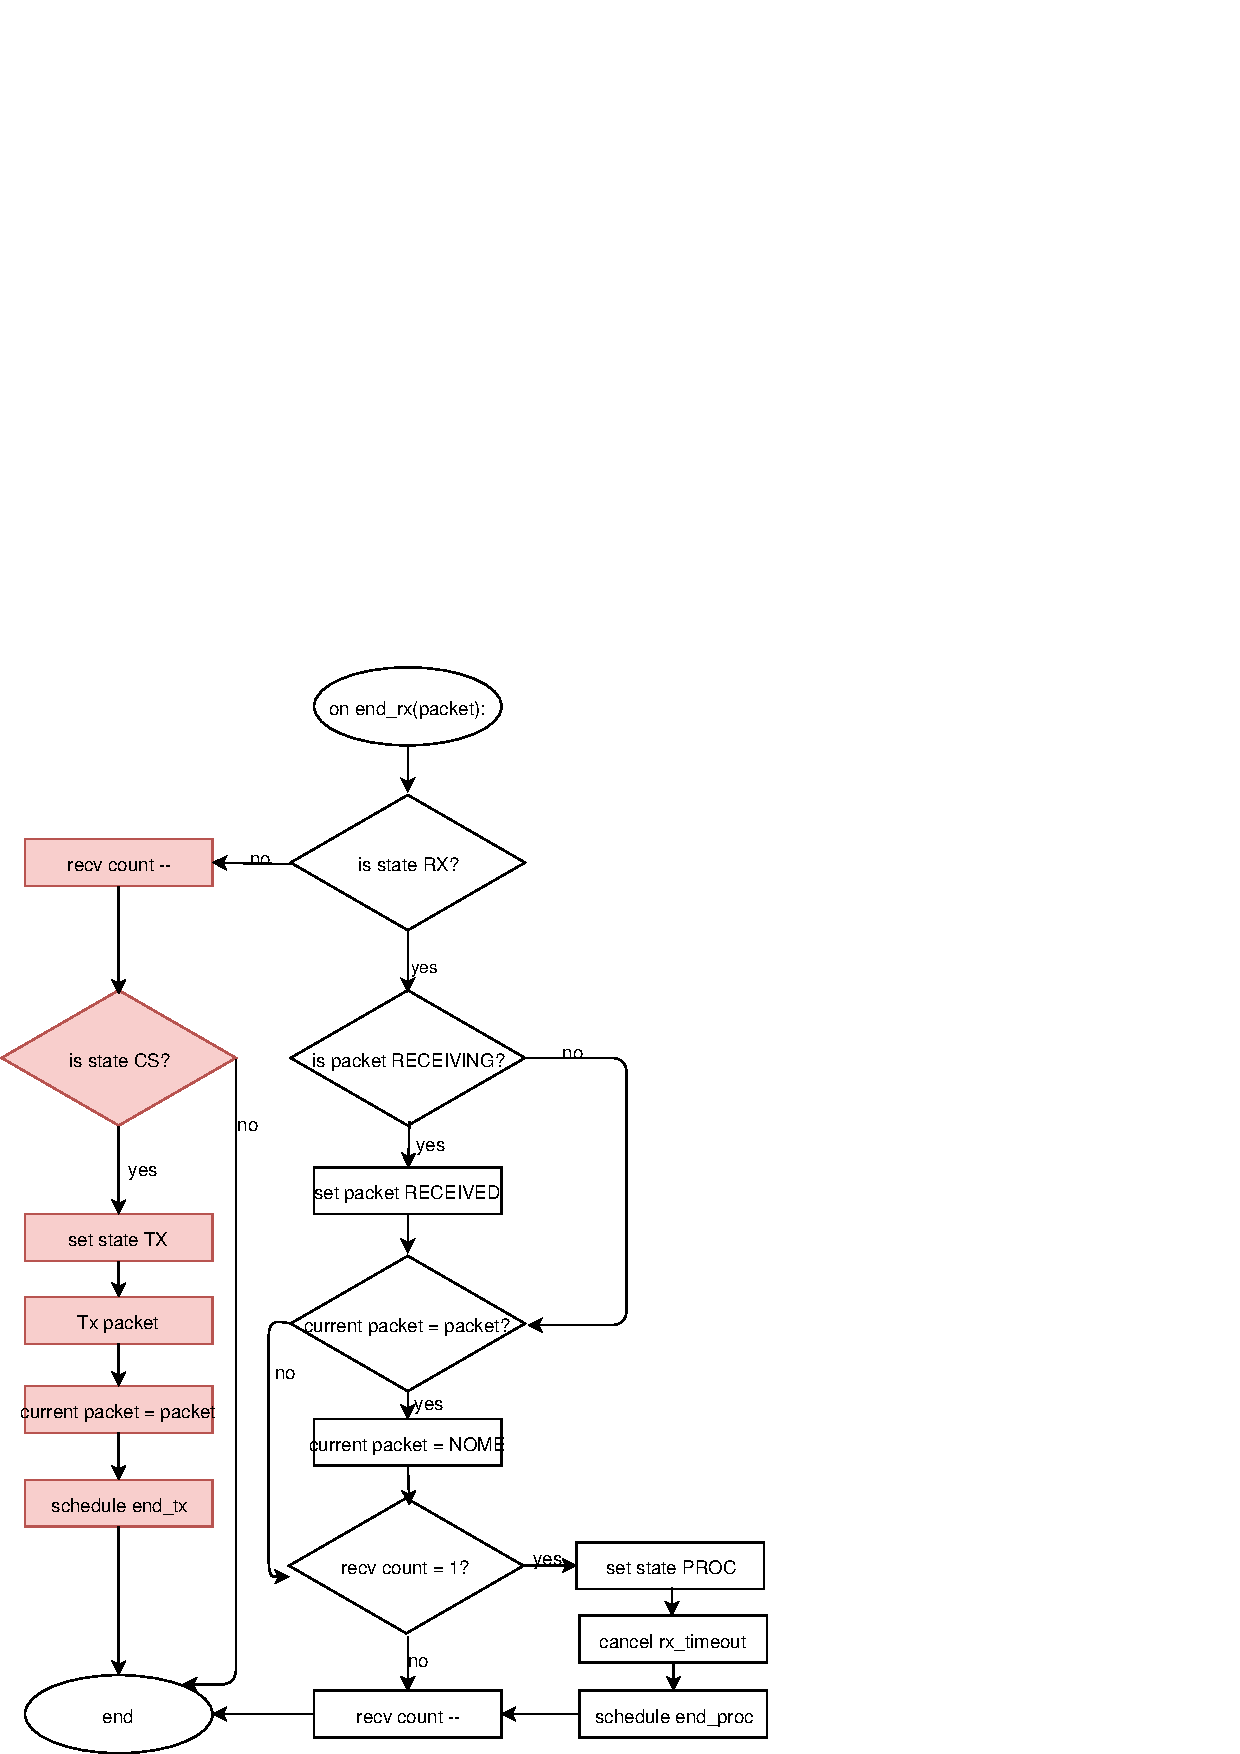
\includegraphics[width=\columnwidth]{figures/end_rx.pdf}}
	\caption{end-RX event}%
\end{figure}

The last event changed is \textit{on-Arrival}, visible on Figure 5, this event happens when a new packet is generated by a node. The modification in this event is concentrated on \textit{IDDLE} state,  if a new packet is generated and  there is not any signal in the air, then the state is changed to \textit{TX}, but if there is some signal in the air, the packet just arrived is put in the queue and then the state is changed to \textit{CS}. Once time on \textit{CS}, the state is changed only there is no signal on air.

\begin{figure}[H]
	\centering	 
	\subfloat{\label{fig:oa}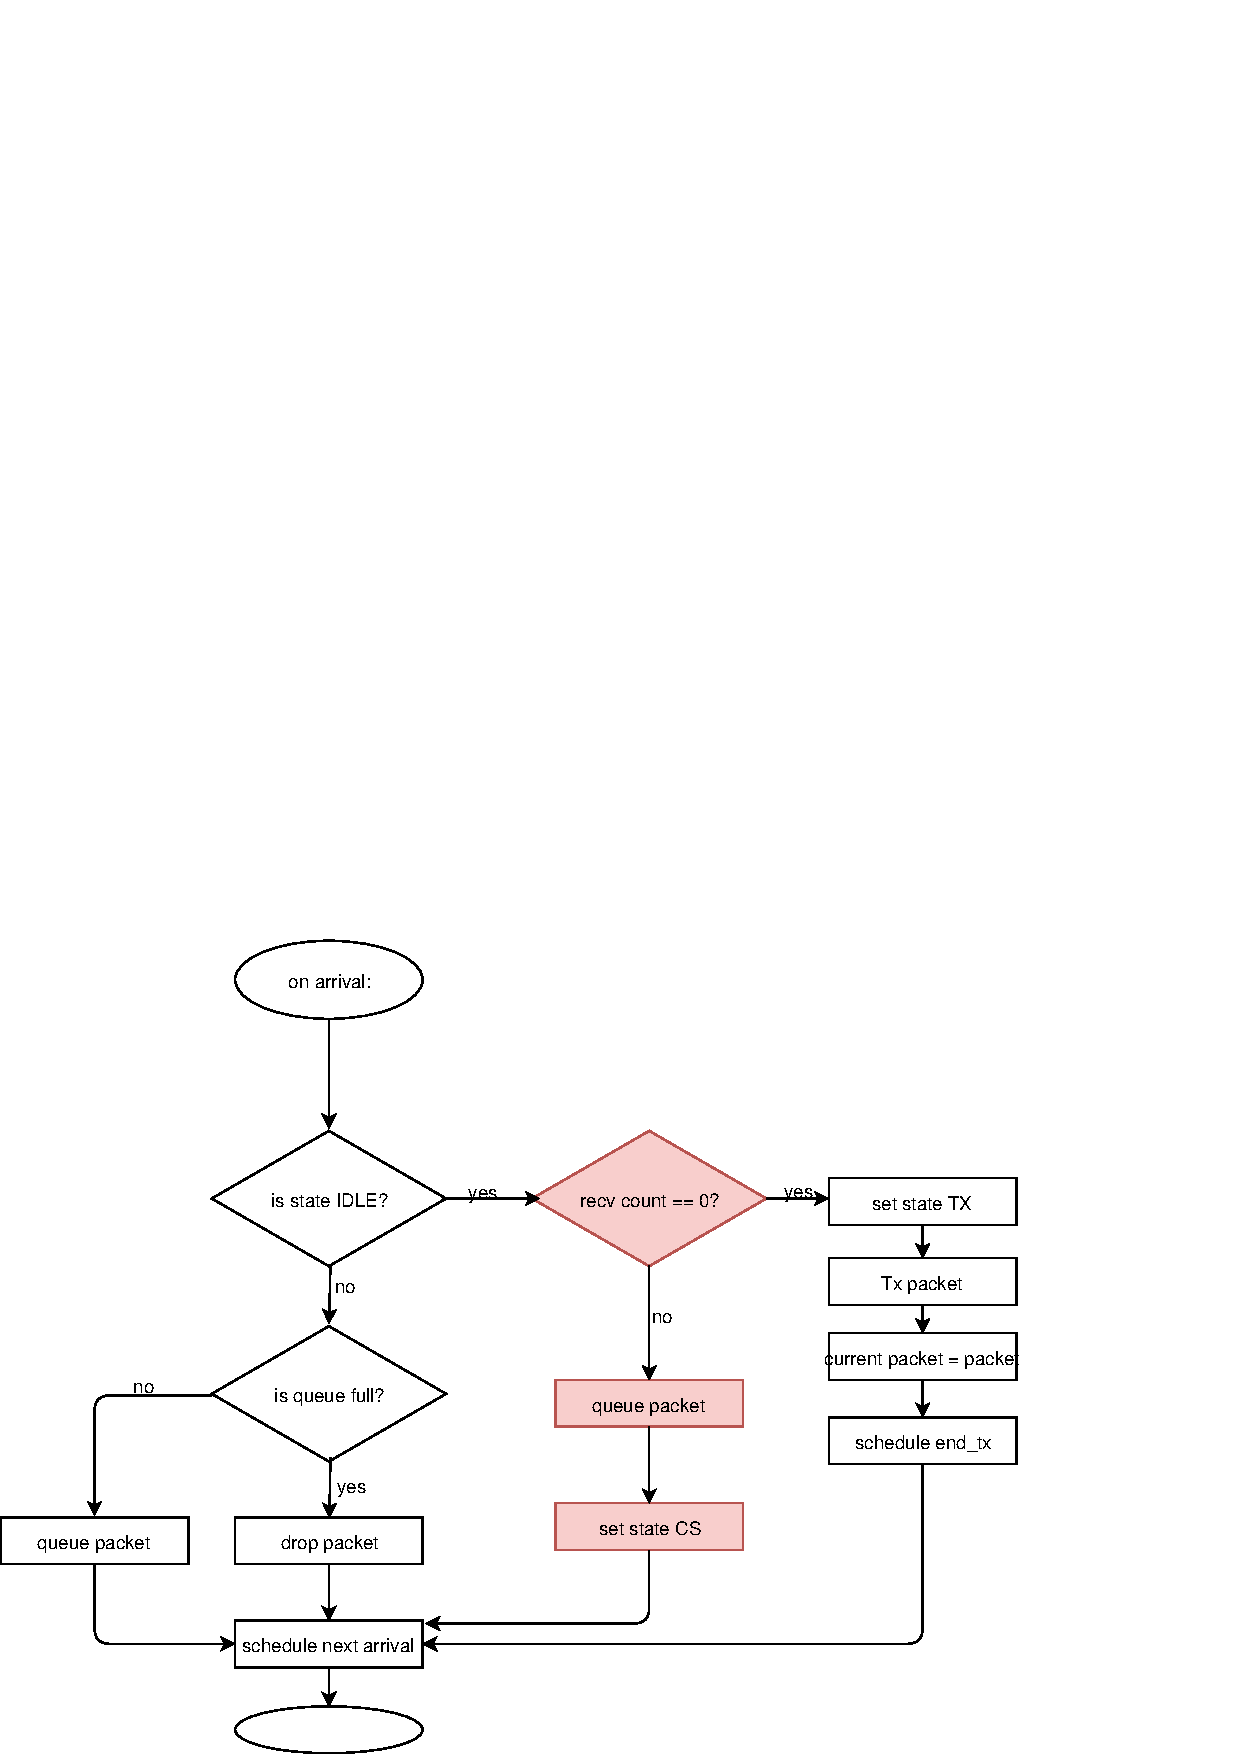
\includegraphics[width=\columnwidth]{figures/on_arrival.pdf}}
	\caption{on-Arrival event}%
\end{figure}


\section{Evaluation}

The evaluation is divided in two parts, the first one represents the results of Simulator Extension, the second one represents the comparison between the base and extension Simulator. The evaluation is made by throughput and packet collision rate at receiver and packet drop rate at sender. 

\subsection{Simulator Extension}

The graph on Figure 6 represents the throughput at receiver by the total offered load. Is interesting highlight the result at receiver 3 and 8. Is possible see on Figure 1 their network position. The receiver node 3 is clearly the more remote node in the network, instead the node 8 is the node with more neighbours near. Is possible in the Figure 6 that when the throughput decrease for the nodes 1-2,4-10 \textit{more quickly for the node 8}, the throughput increases for the node 3. Been the node 3 more distance of others nodes, the rate of packet collision and drop is less than of theirs, it allows the throughput to grow in when others nodes decrease.


\begin{figure}[H]
	\centering	 
	\subfloat{\label{fig:rp1}\includegraphics[width=\columnwidth]{figures/thr_10.pdf}}
	\caption{Throughput Simulator Extension}%
\end{figure}

The graph on Figure 7 represents the packet collision rate by the total offered load. Another time focus is on receiver 3 and 8. The receiver 3 has clearly the rate lowest, instead the node 8 has the highest. The node range in the network is 10 meters, the node 3 is seen only by the node 6. its allows the node 3 has a less packet collision rate.

\begin{figure}[H]
	\centering	 
	\subfloat{\label{fig:rp3}\includegraphics[width=\columnwidth]{figures/pcr_10.pdf}}
	\caption{packet collision Simulator Extension}%
\end{figure}

The graph on Figure 8 represents the packet dropped rate by the total offered load. Here another the the nodes 3 and 8 are distinct. The packet drop rate reflects the time the protocol is in the \textit{CS} state.
 
\begin{figure}[H]
	\centering	 
	\subfloat{\label{fig:rp5}\includegraphics[width=\columnwidth]{figures/pdr_10.pdf}}
	\caption{packet dropped Simulator Extension}%
\end{figure}

\subsection{Comparison between base and extension Simulator}
The Figure 9 represents the throughput at receiver, is possible see that the extension version has a slight more peak than the base version. The reason is that there are already nodes in the \textit{CS} state, allowing the other nodes to transmit  without collision, the throughput decrease after the highest peak, probably the reason  is that all nodes are in the state \textit{CS}, after which the throughput returns to increase in relation to the base version, probably because the nodes try to retransmission.

 \begin{figure}[H]
	\centering	 
	\subfloat{\label{fig:rp15}\includegraphics[width=\columnwidth]{figures/ALLthr.pdf}}
	\caption{Throughput}%
\end{figure}


The Figure 10 represents the packet collision at receiver. The extension version has a mean slightly lower than the base version. The reason is that when the protocol is in the state \textit{CS}, the node stop transmitting, decreasing the collision.

\begin{figure}[H]
	\centering	 
	\subfloat{\label{fig:rp15}\includegraphics[width=\columnwidth]{figures/ALLpcr_.pdf}}
	\caption{packet collision}%
\end{figure}


The Figure 10 represents the packet dropped at sender, is possible to see that the mean of extension version is greater than the base version, it happens  because when the protocol is \textit{CS} state, when new packets arrives they are dropped.

\begin{figure}[H]
	\centering	 
	\subfloat{\label{fig:rp15}\includegraphics[width=\columnwidth]{figures/ALLpdr_.pdf}}
	\caption{packet dropped}%
\end{figure}

\section{Conclusion}
The extension of the protocol with trivial Carrier Sensing allowed to decrease the collision rate, in addition to increasing the throughput, the trivial Carrier Sensing implemented in this project does not contain \textit{slotted aloha} methodology, being one of the reasons that caused the average packet dropped to be high in respect to the base version.
\end{document}
